\documentclass[parskip=half]{scrartcl}
	
\usepackage[english]{babel}
\usepackage[latin1]{inputenc}
\usepackage{enumerate} % til \begin{enumerate}[(i)]
\usepackage{enumitem} % til at styre lister globalt
\usepackage{latexsym} % symboler
\usepackage{amsthm} % til thm osv
\usepackage{amssymb} % flere symbloer
\usepackage{bm} % bold math symbols
\usepackage{amsmath} % til pmatrix
\usepackage[hyphens]{url} %til \url med bindestreger
%\PassOptionsToPackage{hyphens}{url}\usepackage{hyperref}
\usepackage[pdftex]{graphicx}	
\usepackage{scrlayer-scrpage} % page setup

\usepackage{framed}
\usepackage[cache=false]{minted} % for source code
%\usepackage{xcolor}
%set page header
\chead{FYS-STK4155 --- project 3}


% List will number things using (a), (b), ...
\setenumerate[1]{label={(\alph*)}} % Global setting

% Title setup
\title{Report for project 3}
\date{\today}
\author{Jon Audun, Mikael Ravndal and Adam P W S{\o}rensen}

\newcommand{\setof}[2]{\left\{ #1 \; \middle\vert \; #2 \right\}}

\DeclareMathOperator{\cspan}{\overline{span}}

% Theorem opsætning
\newtheorem{theorem}{Theorem}[section]
\newtheorem*{theorem*}{Theorem}
\newtheorem{lemma}[theorem]{Lemma}
\newtheorem{corollary}[theorem]{Corollary}
\newtheorem{proposition}[theorem]{Proposition}
\newtheorem{example}[theorem]{Example}
\newtheorem{conjecture}[theorem]{Conjecture}
\theoremstyle{definition}
\newtheorem{definition}[theorem]{Definition}
\newtheorem{assumption}[theorem]{Standing Assumption}
\newtheorem*{assumption*}{Standing Assumption}
\theoremstyle{remark}
\newtheorem{remark}[theorem]{Remark}
\newtheorem{notation}[theorem]{Notation}

%%%%%%%%%%%%
% notation short cuts
\newcommand{\vect}[1]{{\bm{#1}}}
\newcommand{\funcname}[1]{{\color{blue}{\texttt{#1}}}}
\newcommand{\varname}[1]{\texttt{#1}}
%%%%%%%%%%%%
% bb letters
\newcommand{\C}{\mathbb{C}}
\newcommand{\E}{\mathbb{E}}
\newcommand{\N}{\mathbb{N}}
\newcommand{\Q}{\mathbb{Q}}
\newcommand{\R}{\mathbb{R}}
\newcommand{\Z}{\mathbb{Z}}
% cal letters
\newcommand{\A}{\mathcal{A}}
\newcommand{\B}{\mathcal{B}}
\newcommand{\D}{\mathcal{D}}
\newcommand{\cL}{\mathcal{L}}
\newcommand{\M}{\mathcal{M}}
\newcommand{\cZ}{\mathcal{Z}}
% frak letters
\newcommand{\fA}{\mathfrak{A}}


%%%%%%%%%%%%%%
\begin{document}
%%%%%%%%%%%%%%

\maketitle

\begin{abstract}
In this project we analysed some cooking data and did fairly well. 
\end{abstract}


\section{Introduction}
The concept of machine learning have gained a hughe popularity boost over 
the last couple of years. And this is no wonder: the techniques 
have a wide range of applications and can be a major asset
if you know when to use what.
\par
When to use what is exactly what we're going to have a brief
peek into in this project. 
We will evaluate the performance of three different methods for
classification on a data set consisting of recipies labeled with 
the cuisines they belongs to. That is we are looking at a classification 
problem with multiple classes. The methods we will look at are
logistic regression, support vector machines and random forests.
\begin{framed}
All the code we have implemented can be found at \url{https://github.com/???}.
A print of the jupyter notebook is also attached at the end of this report.
\end{framed}

\section{Methods} \label{sec:methods}
First we need to establish some notation. In the following we assume
that we are given $N \in \N$ samples consisting of $p \in \N$ features
and one target. Further we let $K \in \N$ be the number of
classes in our classification problem. We then denote by $x_{i,j}$ the
$j$-th feature of the $i$-th sample and by $t_i \in \{1,2, \dots, K\}$
the target of the $i$-th sample. 

\subsection{Logistic Regression}
%Logistic regression might be considered the oldest of the three methods
%we compare, as it is based on the logistic funtion which first was
%described back in the 19th century \cite{1}.
Let $\bm{x}_i := (1, x_{i,1}, x_{i,2}, \dots, x_{i,p})$ 
be the row-vector in $\R^{p+1}$ consisting of a one followed by the 
features of sample $i$. Also let $\bm{\beta_k}$ be a column-vector in 
$\R^{p+1}$ for $k \in \{1,2, \dots, K-1\}$ and let 
$\bm{\theta} := [\bm{\beta}_1 \ \bm{\beta}_2 \ \dots \ \bm{\beta}_{K-1}]$ 
be the matrix with the $\bm{\beta}_k$'s as it's columns.
In the case of multinomial logistic regression our model is then given by
\begin{equation}
    \begin{split}
        P_k(\bm{x}; \bm{\theta}) \ = \ 
        \frac{\exp(\bm{x \beta}_k)}
        {1 + \sum_{l=1}^{K-1} \exp(\bm{x\beta_}l)}
        & \quad \quad k \in \{1,2, \dots, ,K - 1\}  \\
        P_K(\bm{x}; \bm{\theta}) \ = \ 
        \frac{1}
        {1 + \sum_{l=1}^{K-1} \exp(\bm{x\beta_}l)}
    \end{split}
\end{equation}
where the ${\bm{\beta_k}}$'s are the 
coefficients we wish to estimate. $P_k(\bm{x}; \bm{\theta})$ is then the 
probability that a sample with features $\bm{x}$ belongs to category $k$. 
\par
The way we fit our model in the case of logistic regression deviates
slightly from the usual proceedure with the introduction of a 
loss function. We now instead define a function we wish to
maximize, namely the log-likelihood function given by 
\begin{equation}
    L(\bm{\theta}) = \sum_{i=1}^N \sum_{k=1}^K 
    \chi_{\{k\}}(t_i) \log( P_k(\bm{x}_i; \bm{\theta}))
\end{equation}
However the difference doesn't go further than the fact that this function
shouldn't be interpreted exactly as a loss function. 
Other than that we proceed as usual by minimizing the negative of this 
function in order to maximize the original function. To do this we
first need to compute the derivative of this function with respect 
to $\bm{\theta}$. Some computations gives us
\begin{equation}
    \frac{\partial L (\bm{\theta)}}{\partial \beta_{k,j}} \ = \
    \sum_{i=1}^N \chi_{\{k\}}(t_i) x_{i,j} (1 - P_k(x_i ; \theta))
\end{equation}
We are now all set to use the gradient method of your choice to minimize
$-L$ as a function of $\bm{\theta}$.

\subsubsection{Gradient descent}
The perhaps simplest approach to minimizing a real valued function
$f$ iteratively, is to set some starting point $\bm{x}_0$, compute the 
gradient
$\nabla f$ in $\bm{x}_0$, and move $\eta > 0$ in the opposite direction of 
this gradient in order to obtain 
$\bm{x}_1 = \bm{x}_0 - \eta \nabla f(\bm{x}_0)$. Then
one iterates by setting 
$\bm{x}_{i+1} = \bm{x}_i - \eta \nabla f\bm{(}x_0)$ for $i=1,2,...$. 
This is the framework of gradient descent.
For small enough $\eta$ this implies $f(\bm{x}_i) > f(\bm{x}_{i+1})$. 
The problem with this approach is to find out what 
$\eta$ is small enough. If we choose
$\eta$ too small, it might take days for our algorithm to converge. If 
we on the contrary choose $\eta$ to big, it might not converge at all.

\subsubsection{Newton-Raphson}
The Newton-Raphson method is a kind of gradient descent method, 
except we choose the learning rate in a more clever way. We thus 
start out by choosing a random starting point $\bm{x}_0$, just as in the 
case of gradient descent. The update step however is a bit different:
\begin{equation}
    \bm{x}_{i+1} \ = \ \bm{x}_{i} - 
    \frac{\partial^2 f(\bm{x}_i)}{\partial \bm{x}_i \partial \bm{x}_i^T} 
    \frac{\partial f(\bm{x}_i)}{\partial \bm{x}_i}
\end{equation}
The result is a method that converges way faster than normal gradient 
descent. The draw back is however the need to compute the Hessian of 
your objective function. For a thourough derivation of this method 
consult \cite{gradient}

\subsubsection{Stochastic gradient descent}
To avoid overfitting when training neural networks, training on 
randomly picked batches of the training data for each iteration is a good
regularization method. If we let $b$ be our batch size, the first step of
this method consists of dividing the training data into $N//b$ batches. 
One does this by picking from the $N$ data-points without replacement. 
The second step is then to perform a gradient descent as described in 
section 2.1.1 with a new batch for each iteration.

\subsection{\protect
\includegraphics{svmheading.png}}

To call a Support Vector Machine classifier with no kernel we use the following Python code:
\begin{minted}{python}
svm_clf =  svm.LinearSVC(C = 0.1)
svm_clf.fit(x_train, y_train)
preds = svm_clf.fit(x_test)
print('We did this good: %.4f' % accuracy_score(y_test, preds))
\end{minted}

\subsection{Decision trees}
Wikipedias overview on decision trees:
\begin{quotation}
	A decision tree is a flowchart-like structure in which each internal node represents a ``test'' on an attribute (e.g. whether a coin flip comes up heads or tails), each branch represents the outcome of the test, and each leaf node represents a class label (decision taken after computing all attributes). The paths from root to leaf represent classification rules.
\end{quotation}
A decision tree typically uses all of the features as its features. The result of this is then that you get a classifier which predicts well on the training data, but falls short on testing data. This is because it fits its classifier perfectly to the data which it has seen. So a lone decision tree with all features will almost always be overfitted.
\subsubsection{Rather a forest, then just a tree}
This is why random forests are more popular. A random forest can usually generalise much better then what a lone tree can.\\
A random forest is constructed by choosing how many decision trees you want in the forest and then train every tree on your data. But the construction of these trees is done differently then a lone decision tree.\\
\\
Each tree just use a subset of the features, typically $ features = \sqrt{all-features}$. This makes it so each tree functions a bit differently and will then predict different things.\\
The final prediction then becomes which of the classes which gets voted most for when every tree predicts their own.
\subsubsection{Difference in number of trees}
The number of trees in the forest is the main hyper parameter we have used to tweak this classifier. But it seems like the rule of thumb was the more, the merrier.
Here is a plot of how well the random forest did:\\
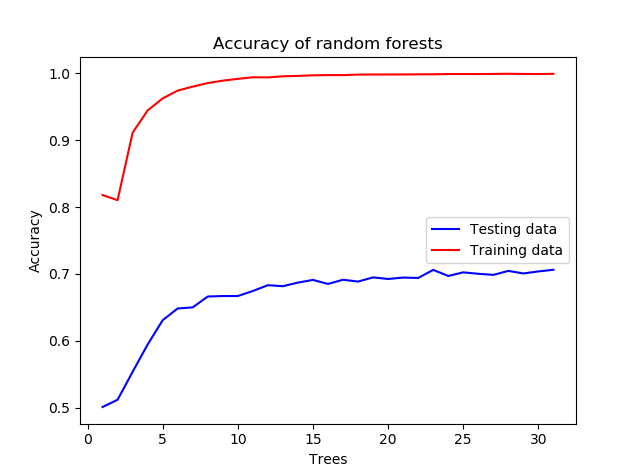
\includegraphics[scale=.7]{images/32treesAcc}\\
So more trees provides a better accuracy. But the classifier starts to have a decent accuracy after 10 trees.

\subsubsection{Difference in number of max\_features}
Here is a plot on how well the accuracy is using different numbers as max\_features:\\
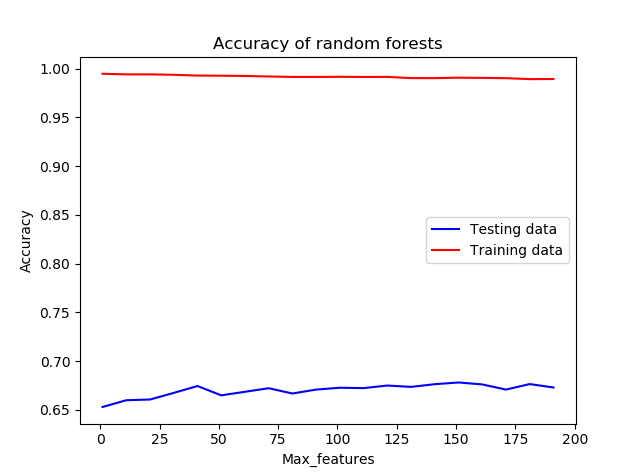
\includegraphics[scale=.7]{images/Max_featuresplot}\\
The number of trees used is 10.\\
\\
The default in the scikitlearn classifier is using the root of the number of all the features as max\_features. Since we have approximately 2000 features, the root becomes 44.72. That's why I computed different accuracies around this number.\\
\\
The plot tells us that it doesn't seem to matter much what we use as max\_features. The optimum in the plot is around 40 which gives us just more reason to stick with the default of using the root of all the features as max\_features.

\section{Model Selection and Verification}

\section{Results} \label{sec:results}

\section{Conclusion} \label{sec:conclusion}

We did good.

%%%%%%%%%%%%%%
%Bibliography
\bibliographystyle{apalike}
\bibliography{refs}	% expects file "refs.bib"
%%%%%%%%%%%%%%


\end{document}
